\section{Matching}
\label{sec:matching}

\subsection{Features}
\label{subsec:the-features}

Before diving deeper into the matching algorithm, it's important to explain the features that are used to do the matching. One possibility is to use keypoints detected by algorithms like SURF \cite{bay2006surf} or ORB \cite{rublee2011orb}. However, keypoints turn out to be inefficient and inappropriate for object detection in museums \cite{bay2006interactive}.

The algorithm in this document only depends on two types of histograms from the detected paintings. The first type is a histogram of the full painting, the second type is a collection of histograms gathered from different blocks of the painting. The block size used in this algorithm divides the painting in 4 rows by 4 columns (or 16 blocks), independent of the painting's size. Both features are saved to the database for each of the labeled paintings and are both used in the matching algorithm explained in the next section.

\subsection{The matching algorithm}
\label{subsec:matching-algo}

The first step in matching a given painting with the entire dataset of paintings is a light intensity equalization. This way different light intensities have no influence on the histograms gathered from a detected painting. Equalization is a technique that is only used on the video frames because of the rather bad frame quality, the dataset itself and the previously performed benchmarks don't need this step. \cite{patel2013comparative}

The second step consists of fetching the histograms as described in \sectionref{subsec:the-features}. Thereafter these histograms are compared against all histograms in the dataset. Per known painting, the distance between the histograms is calculated using a technique called \emph{correlation}. This way a chance between 0 and 1 is obtained. The histogram of the whole painting gives one chance, the block histogram gives a total of 16 chances which are combined by taking the average. These two chances are combined using \formularef{eq:histogram-score} which calculates a weighted average. In this formula, $P(X = P_{i})$ stands for the chance that the detected painting $X$ is painting $P_{i}$ from the dataset, $B$ stands for the average of the block histogram distances and $F$ stands for the distance of the normal histograms. The block histogram gets a much higher weight because the predictions with these histograms are much more reliable than these with the normal histograms.

\begin{equation}
    \label{eq:histogram-score}
    P(X = P_{i}) = \frac{(8 * B) + (1 * F)}{9}
\end{equation}

The matching algorithm gives a list of possible rooms with the according chances per detected painting, even if the room is not accessible given the current room. How impossible rooms are treated, will be explained in \sectionref{sec:localization}. The algorithm has also an option to ignore matches that are below a given threshold.

\subsection{Matching results}
The matching algorithm has been tested in three ways. First, the dataset was matched against itself without using the detection algorithm but by using the corners from the semi-supervised algorithm. This test uniquely matched 835 of 836 paintings correctly. This means that only one painting could not be uniquely matched, this could be because some paintings appear in multiple images. The average matching probability is 92.24\%.

The second test was performed on the dataset in combination with the detection algorithm described in \sectionref{subsec:detection-algo}. This test indicates that 702 of the 762 detected paintings were matched correctly. These results are displayed on the graphs in \figureref{fig:correct-incorrect-paintings}.

The third and last test was performed on the test dataset also in combination with the detection algorithm. The images have been divided into folders with the correct room as name to be able to count the number of correct room matches. This test reveals that 158 of the 338 detected paintings had a correct room match. This is lower than the dataset because these images are meant to be more difficult to match because of the angle, rotation, light intensity, etc.

\begin{figure}
    \centering
    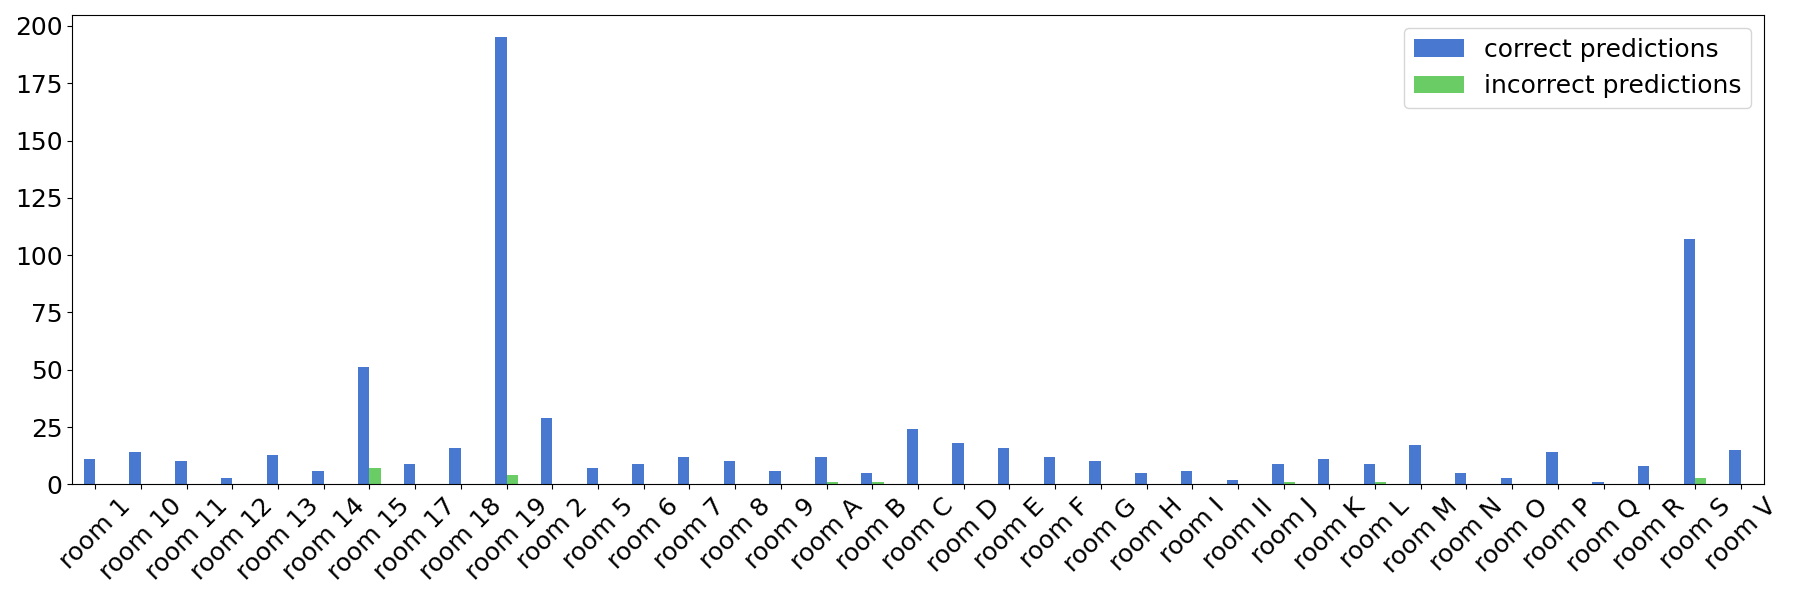
\includegraphics[width=\linewidth]{correct_and_incorrect.png}

    \caption{Correct and incorrect painting predictions per room}
    \label{fig:correct-incorrect-paintings}
\end{figure}
